\section{Треугольники и четырёхугольники}

В абсолютной геометрии доказывается ряд утверждений, каждое из которых равносильно аксиоме параллельности Евклида: сумма углов треугольника равна $2d$, точки, равноудалённые от прямой, лежат на прямой (предложение Посидония), перпендикуляр к стороне острого угла пересекает другую сторону (предложение Лежандра), около любого треугольника можно описать окружность~[2]. В геометрии Лобачевского выполняются их отрицания. В этом разделе они доказываются и интерпретируются в модели.

\subsection{Сумма углов треугольника}

\begin{definition}
Четырёхугольник $ABCD$, у которого углы при стороне $AB$ прямые, называется \emph{двупрямоугольником} с основанием $AB$. Если, кроме того, $AD=BC$, он называется \emph{четырёхугольником Саккери}, а сторона $CD$~--- его верхним основанием.
\end{definition}

\begin{lemma}\label{lem:sakkeri-ravny}
В абсолютной геометрии углы четырёхугольника Саккери при верхнем основании равны.
\end{lemma}
\begin{proof}
Прямоугольные треугольники $ABD$ и $BAC$ равны по двум катетам ($AB$ общий, $AD=BC$), поэтому $BD=AC$. Тогда треугольники $ADC$ и $BCD$ равны по трём сторонам, и $\angle ADC=\angle BCD$.
\end{proof}

\begin{lemma}\label{lem:treugolnik-sakkeri}
Для любого треугольника $ABC$ существует четырёхугольник Саккери, сумма углов при верхнем основании которого равна сумме углов треугольника.
\end{lemma}
\begin{proof}
Пусть $M$ и $N$~--- середины сторон $AB$ и $AC$. Опустим на прямую $MN$ перпендикуляры $AA'$, $BB'$, $CC'$. Прямоугольные треугольники $AA'M$ и $BB'M$ равны по гипотенузе и острому углу, поэтому $BB'=AA'$ и $\angle B'BM=\angle A'AM$. Точно так же $CC'=AA'$ и $\angle C'CN=\angle A'AN$. Значит, $B'C'CB$~--- четырёхугольник Саккери с основанием $B'C'$. Если точка $A'$ лежит между $B'$ и $C'$, то
\[
\angle B'BC+\angle C'CB=(\angle A'AB+\angle B)+(\angle A'AC+\angle C)=\angle A+\angle B+\angle C.
\]
Остальные случаи расположения точки $A'$ разбираются так же, только одно из слагаемых $\angle A'AB$, $\angle A'AC$ входит со знаком минус.
\end{proof}

Нам понадобятся две теоремы абсолютной геометрии, доказательства которых приведены в~[2].

\begin{theorem}[первая теорема Лежандра]\label{thm:lezhandr1}
Сумма углов любого треугольника не превосходит $2d$.
\end{theorem}

\begin{theorem}[вторая теорема Лежандра]\label{thm:lezhandr2}
Если сумма углов хотя бы одного треугольника равна $2d$, то выполняется аксиома параллельности Евклида.
\end{theorem}

\begin{lemma}\label{lem:sakkeri-ostrye}
В геометрии Лобачевского углы четырёхугольника Саккери при верхнем основании острые.
\end{lemma}
\begin{proof}
Диагональ делит четырёхугольник на два треугольника, поэтому по теореме~\ref{thm:lezhandr1} сумма его углов не больше $4d$. Углы при основании прямые, углы при верхнем основании по лемме~\ref{lem:sakkeri-ravny} равны, значит, каждый из них не больше $d$. Если бы они были прямыми, то диагональ разбила бы прямоугольник на два треугольника с общей суммой углов $4d$, и по теореме~\ref{thm:lezhandr1} сумма углов каждого была бы равна $2d$. По теореме~\ref{thm:lezhandr2} это противоречит аксиоме Лобачевского.
\end{proof}

\begin{theorem}\label{thm:summa}
На плоскости Лобачевского сумма углов любого треугольника меньше $2d$.
\end{theorem}
\begin{proof}
По лемме~\ref{lem:treugolnik-sakkeri} сумма углов треугольника равна сумме двух углов при верхнем основании некоторого четырёхугольника Саккери, а по лемме~\ref{lem:sakkeri-ostrye} каждый из этих углов меньше $d$.
\end{proof}

Число $\delta=2d-(\alpha+\beta+\gamma)$ называется \emph{дефектом} треугольника. Площадь треугольника пропорциональна дефекту~[4]; при выбранной единице длины, когда радиус кривизны равен $1$, площадь равна $\delta$. Отсюда площадь любого треугольника меньше $\pi$. Из леммы~\ref{lem:sakkeri-ostrye} следует, что на плоскости Лобачевского нет прямоугольников, а из теоремы~\ref{thm:summa}~--- что треугольники с соответственно равными углами равны~[1]. Подобных, но не равных фигур в геометрии Лобачевского нет.

\subsection{Четырёхугольник Саккери в модели}

Поместим основание четырёхугольника Саккери на горизонтальный диаметр симметрично относительно центра: $A=(-p,0)$, $B=(p,0)$. По лемме~\ref{lem:polyus} перпендикуляры к диаметру в точках $A$ и $B$ изображаются вертикальными хордами, поэтому $D=(-p,q)$ и $C=(p,q)$ (рисунок~\ref{fig:sakkeri}). Обозначим длину основания через $b$, а длину боковых сторон через $h$. По следствию~\ref{cor:ot-centra} $p=\thh(b/2)$, а по формуле~\eqref{eq:do-diametra} $\thh h=q/\sqrt{1-p^2}$.

\begin{figure}[H]
\centering
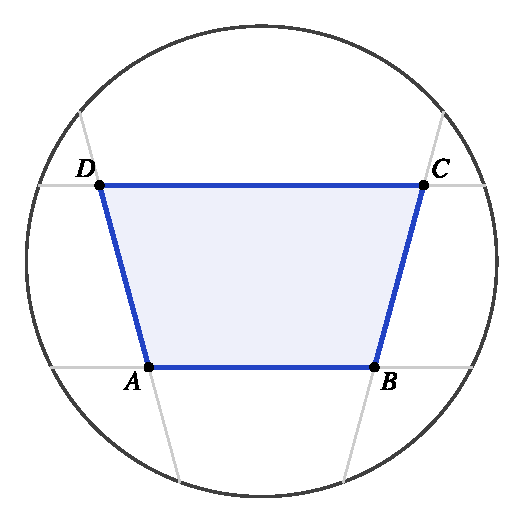
\includegraphics[width=0.46\textwidth]{fig/sakkeri.pdf}
\caption{Четырёхугольник Саккери в модели, перенесённый π-движением вниз. На рисунке он выглядит евклидовой трапецией, углы при верхнем основании равны $54{,}3^\circ$ ($b=1{,}2$, $h=1{,}1$)}
\label{fig:sakkeri}
\end{figure}

\begin{proposition}\label{prop:sakkeri}
Угол $\gamma$ четырёхугольника Саккери при верхнем основании находится по формуле
\begin{equation}\label{eq:sakkeri}
\cos\gamma=\frac{\sh\frac b2\,\sh h}{\sqrt{\ch^2\frac b2+\sh^2\frac b2\,\sh^2h}}.
\end{equation}
\end{proposition}
\begin{proof}
Прямая $BC$ имеет уравнение $k_1-p=0$ и полюс $P_1=(p:1:0)$, прямая $CD$~--- уравнение $k_2-q=0$ и полюс $P_2=(q:0:1)$. По предложению~\ref{prop:ugol}
\[
|\cos\gamma|=\frac{pq}{\sqrt{(1-p^2)(1-q^2)}}.
\]
Угол $\gamma$ острый (лемма~\ref{lem:sakkeri-ostrye}), поэтому знак модуля можно снять. Подставим $p=\thh\frac b2$ и $q=\thh h/\ch\frac b2$; после умножения числителя и знаменателя на $\ch\frac b2\,\ch h$ и замены $\ch^2h=1+\sh^2h$ получается~\eqref{eq:sakkeri}.
\end{proof}

Формула показывает больше, чем утверждение об остроте углов. При $b\to0$ или $h\to0$ угол $\gamma$ стремится к прямому: маленький четырёхугольник Саккери почти неотличим от прямоугольника. При $h\to\infty$ угол стремится к нулю. Числа на рисунке~\ref{fig:sakkeri} получены по этой формуле и совпадают с тем, что показывает сцена «Двупрямоугольник и четырёхугольник Саккери» интерактивной модели.

\subsection{Точки, равноудалённые от прямой}

\begin{definition}[\!\!{[1]}]
Множество точек одной полуплоскости, удалённых от её граничной прямой $a$ на одно и то же расстояние $h$, называется \emph{эквидистантой} с базой $a$ и высотой $h$.
\end{definition}

\begin{proposition}\label{prop:ekvidistanta}
Если база~--- диаметр $k_2=0$, эквидистанта высоты $h$ изображается дугой эллипса
\[
y=\thh h\,\sqrt{1-x^2},\qquad |x|<1,
\]
с полуосями $1$ и $\thh h$. Она не является прямой.
\end{proposition}
\begin{proof}
Уравнение получается из~\eqref{eq:do-diametra}, если положить $d=h$ и $y>0$. Три её точки с абсциссами $0$ и $\pm\frac12$ не лежат на одной хорде: средняя расположена выше хорды, соединяющей крайние, так как функция $\sqrt{1-x^2}$ строго вогнута.
\end{proof}

Это интерпретация отрицания предложения Посидония (рисунок~\ref{fig:ekvidistanta}). Концы эквидистанты совпадают с концами базы, поэтому эквидистанта, в отличие от прямой, параллельной базе, не уходит от неё и не приближается к ней.

\begin{figure}[H]
\centering
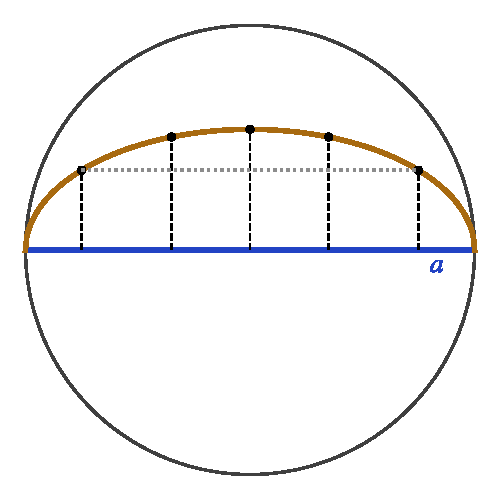
\includegraphics[width=0.46\textwidth]{fig/ekvidistanta.pdf}
\caption{Эквидистанта высоты $0{,}6$ с базой $a$ и перпендикуляры к базе равной длины; пунктир~--- хорда через две точки эквидистанты}
\label{fig:ekvidistanta}
\end{figure}

\subsection{Перпендикуляр к стороне острого угла}

\begin{proposition}\label{prop:lezhandr}
Пусть угол $E_1OE_2$ острый и равен $\varphi$, $P$~--- точка на стороне $OE_1$, $x=OP$. Перпендикуляр к $OE_1$ в точке $P$ пересекает сторону $OE_2$ тогда и только тогда, когда $\Pi(x)>\varphi$. Граничная точка $P^*$, для которой $\Pi(OP^*)=\varphi$, существует для любого острого угла, и перпендикуляр в ней параллелен $OE_2$.
\end{proposition}
\begin{proof}
Поместим вершину $O$ в центр, сторону $OE_1$ на положительную полуось абсцисс, сторону $OE_2$ на луч $t(\cos\varphi,\sin\varphi)$, $0\le t<1$. Угол с вершиной в центре изображается без искажения. По следствию~\ref{cor:ot-centra} точка $P$ изображается точкой $(\thh x,0)$, и по лемме~\ref{lem:polyus} перпендикуляр в ней изображается вертикальной хордой $k_1=\thh x$. Луч $OE_2$ пересекает прямую $k_1=\thh x$ в точке с параметром $t=\thh x/\cos\varphi$, и эта точка лежит в круге тогда и только тогда, когда $\thh x<\cos\varphi$. По теореме~\ref{thm:lobachevsky} $\thh x=\cos\Pi(x)$, поэтому условие равносильно $\Pi(x)>\varphi$. При $\thh x=\cos\varphi$ хорда $k_1=\thh x$ проходит через конец $E_2=(\cos\varphi,\sin\varphi)$ стороны $OE_2$ и по теореме~\ref{thm:parallel-model} параллельна ей.
\end{proof}

Получилось отрицание предложения Лежандра (рисунок~\ref{fig:lezhandr}) и одновременно ещё одно доказательство того, что каждый острый угол является углом параллельности некоторого отрезка. В курсе эти два факта связаны так же: существование отрезка с данным углом параллельности выводится из отрицания предложения Лежандра.

\begin{figure}[H]
\centering
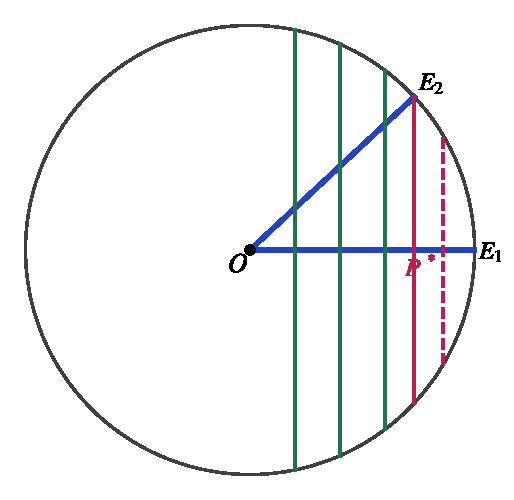
\includegraphics[width=0.46\textwidth]{fig/lezhandr.pdf}
\caption{Перпендикуляры к стороне $OE_1$ острого угла: зелёные пересекают сторону $OE_2$, красный проходит через её конец $E_2$ и ей параллелен, пунктирный её не пересекает}
\label{fig:lezhandr}
\end{figure}

Здесь же видно и отрицание V постулата: прямая $OE_2$ и перпендикуляр в точке $P^*$ не пересекаются, хотя образуют с прямой $OE_1$ внутренние односторонние углы $\varphi$ и $d$, сумма которых меньше $2d$.

\subsection{Треугольник без описанной окружности}

Центр окружности, описанной около треугольника, лежит на серединных перпендикулярах к его сторонам. Поэтому треугольник, у которого два серединных перпендикуляра не пересекаются, окружности не имеет. Пример строится так~[1]. Пусть $a$~--- прямая, $h$~--- перпендикуляр к ней, $A\in h$, и $b$~--- прямая через $A$, не перпендикулярная $h$ и не пересекающая $a$; по теореме~\ref{thm:lv-vsegda} такая прямая существует. Возьмём точку $M\in h$ и отразим её относительно $a$ и $b$, получим точки $N$ и $P$. Тогда $a$ и $b$~--- серединные перпендикуляры к сторонам $MN$ и $MP$ треугольника $MNP$, и они не пересекаются.

В модели все построения выполняются по формулам п.~1.4. На рисунке~\ref{fig:bez-okruzhnosti} прямая $a$~--- горизонтальный диаметр, $h$~--- вертикальный, а прямая $b$ выбрана так, что продолжения хорд $a$ и $b$ пересекаются вне круга; точки $N$ и $P$ получены по формуле~\eqref{eq:otrazhenie}.

\begin{figure}[H]
\centering
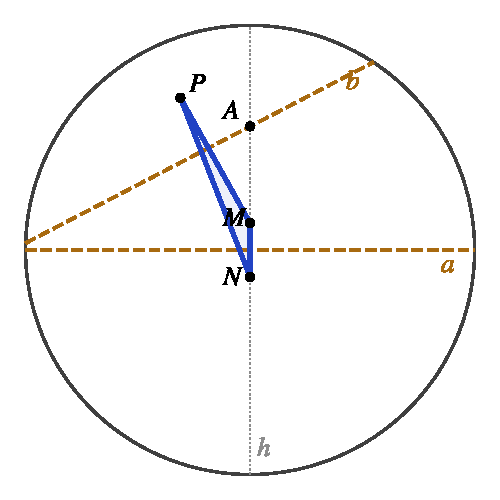
\includegraphics[width=0.46\textwidth]{fig/bez_okruzhnosti.pdf}
\caption{Треугольник $MNP$, серединные перпендикуляры $a$ и $b$ которого расходятся}
\label{fig:bez-okruzhnosti}
\end{figure}

Если же две прямые пересекаются, то любая точка, не лежащая на них, отражённая относительно обеих прямых, даёт треугольник, около которого окружность описать можно.
